% Final study draft. Human interpretation, authorship and submission approval pending.
% Numerical sources: results/revised/analysis/{summary,latency}.json.
\begin{abstract}
Voltage surrogates require a decision rule for invoking an exact solver after a feeder changes. We compare neural, physics-only and physics-augmented routes on a synthetic 33-bus feeder, with 15 development and 44 held-out branch exchanges, three training seeds and three test seeds. At a frozen threshold calibrated for 10\% escalation, a residual model using current LinDistFlow information yields 0.0065\% unsafe approvals and 0.0248\% false rejections, versus 0.0615\% and 0.1678\% for physics-only routing. Realized escalation is 8.40\% versus 8.66\%, but the residual route costs more computation. A 10\% impedance underestimate raises its unsafe rate to 2.24\%; stale topology raises it to 14.86\%. Of 1.83 million generated cases, 2,315 remain numerically unresolved and are excluded from decision-risk denominators. The results support learned correction with current network information, while exposing its calibration and verifier limits.
\keywords{selective prediction, power flow, topology shift,\newline residual learning, calibration, runtime verification}
\end{abstract}

% Draft for author review. No revised outcome claims belong in this section.
\section{Introduction}
\label{sec:introduction}

A voltage surrogate can approve an operating point quickly. The relevant question is whether its decision remains useful after the feeder changes. A learned predictor trained on one network need not receive the information that distinguishes two switch configurations. When that information is absent, repeated predictions on the same loads, photovoltaic injections and slack-voltage setting can remain confident even though the physical voltage profile changes.

Exact power-flow fallback does not settle which points should be checked. Escalating every case removes the computational purpose of the surrogate. Escalating too few can leave unsafe approvals, while rejecting uncertain cases can discard feasible operation. These costs must be measured together. A physics-assisted neural route therefore requires comparison with the same physics model used directly, with exact fallback, to identify what the neural component contributes.

We study this comparison on a synthetic, balanced 33-bus radial feeder. The stale neural ensemble sees operating features but no current topology. LinDistFlow receives the supplied network model. A separate residual predictor also receives the current LinDistFlow voltage extrema and is trained across development topologies. This information difference is intentional and explicit. The study asks when external physics helps a stale predictor and whether a learned correction improves on physics alone. Models with and without topology information are different observers.

The evaluation pairs operating points across every connected radial single branch exchange in the feeder inventory. It separates development exchanges from held-out exchanges, fixes thresholds using independent calibration data and perturbs the verifier while keeping the physical reference unchanged. It preserves unresolved reference solves. These choices distinguish ranking quality, frozen-route transfer and dependence on accurate external information.

\subsection{Related work and scope}

Reject-option prediction formalizes the tradeoff between error and refusal~\cite{chow1970}. Learning to defer extends this setting to a downstream expert~\cite{mozannar2020}, while cascade analysis explains why the first model's confidence need not identify when another model helps~\cite{jitkrittum2023}. Deep ensembles motivate a spread diagnostic~\cite{lakshminarayanan2017}; the present member-margin spread is not a reproduction of every component of that method. Calibrate-Then-Delegate studies risk and budget guarantees for cascades~\cite{pona2026}. Our local probes do not implement those guarantees. We instead include a separate split-conformal margin interval and state its exchangeability requirement~\cite{angelopoulos2023}.

Combining a complex learned component with simpler verification has an established architectural history~\cite{sha2001}. Power-system research also addresses feasibility directly. DeepOPF+ calibrates constraints during training~\cite{zhao2020}, and Venzke et al. study worst-case guarantees for neural optimal power flow~\cite{venzke2020}. Parker constructs adversarial AC-power-flow inputs that distinguish surrogate feasibility from physical feasibility~\cite{parker2026}. These results motivate checking decisions against the governing equations rather than interpreting predictive confidence as a feasibility certificate.

Exact fallback is already part of this literature. Shamseldein combines learned AC feasibility, conformal prediction and an exact Newton--Raphson solver~\cite{shamseldein2026}. Nawaz et al. describe physics-informed graph surrogates with residual-triggered Newton--Raphson fallback and topology perturbation tests~\cite{nawaz2026}. Our contribution is therefore a controlled comparison of routing choices and their information requirements, not the first use of physics or exact fallback. Its scope is one feeder family, specified synthetic operating distributions and enumerated branch exchanges. Any advantage must survive comparison with physics-only routes, false-rejection accounting and measured computation.

% Draft based on protocol/PROTOCOL.md and amendment 1, read 2026-09-22.
% Parent must reconcile final completed-run details and supply actual results.
\section{Benchmark and routing methods}
\label{sec:methods}

\subsection{Voltage decision and information}

The feeder uses the 33-bus data associated with Baran and Wu~\cite{baran1989reconfiguration}. The task is a voltage-band decision under a balanced steady-state model, not dispatch optimization or a field-safety claim. For voltage magnitudes $v$, define
\begin{equation}
 m(v)=\min\!\left\{\min_i v_i-0.95,\;1.05-\max_i v_i\right\}.
 \label{eq:margin}
\end{equation}
A resolved reference point is feasible when $m(v)\geq0$. The neural margin $m_N$ uses the ensemble-mean minimum and maximum voltages. The spread $\sigma$ is the sample standard deviation of the five individual member margins. LinDistFlow supplies a margin $m_L$ from approximate voltage drops on the supplied radial network~\cite{baran1989reconfiguration,turitsyn2011}.

The 71 operating features comprise 32 active and 32 reactive loads, six photovoltaic outputs and the slack voltage. They exclude topology. The nominal generator samples a global load multiplier in $[0.3,1.1]$, per-bus multipliers in $[0.7,1.3]$ and slack voltage in $[0.97,1.05]$ pu. Photovoltaic output is zero with probability $0.25$; otherwise irradiance, plant scaling and retained output are sampled independently within the recorded configuration. A secondary original-topology test raises photovoltaic ratings by $60\%$ and uses global load multipliers in $[0.2,0.8]$.

\subsection{Training and topology allocation}

Three training seeds each generate 30,000 nominal-topology training points, 10,000 separate probe-training points and 10,000 threshold-calibration points. Each ensemble contains five independently initialized ReLU networks with two 32-unit layers. Networks use Adam, batch size 256, learning rate $10^{-3}$ and at most 250 epochs. Early stopping uses a 10\% internal validation split, patience of 25 epochs and tolerance $10^{-7}$. Input and regression-target scalers are fitted on training data. Stopping histories and warnings are retained.

The inventory contains 59 connected radial nonbaseline single branch exchanges. Fifteen are development topologies, including the two exchanges examined during the exploratory study; the remaining 13 development exchanges follow a recorded hash rule. The other 44 exchanges form the primary held-out set. This protocol was frozen after exploratory analysis, not preregistered before any observation.

A physics-augmented residual network uses two 64-unit layers and the same optimizer and stopping settings. Let $\ell$ contain the supplied minimum and maximum LinDistFlow voltages. The corrected prediction is
\begin{equation}
 \hat y_R(x,\ell)=\ell+h_\theta([x,\ell]).
 \label{eq:residual}
\end{equation}
The network fits standardized exact-minus-linear extrema by squared-error regression. Its corrected extrema define margin $m_R$. Each training seed uses 3,000 points from each development topology and 3,000 from the original topology, for 48,000 points. Held-out-topology labels enter neither fitting nor calibration. This baseline receives current-physics information rather than an explicit graph encoding, and its additional training data are reported as a cost.

Three independent test seeds generate 10,000 operating points each, paired across the original feeder and all 59 exchanges. Three further nominal-topology photovoltaic-growth sets give 1,830,000 generated topology--scenario pairs. Reuse across training runs and verifier variants does not create additional independent labels. The three training runs crossed with three test draws yield nine model--test combinations per condition.

\subsection{Routes and frozen thresholds}

A route combines a provisional verdict with a score; larger scores receive exact evaluation first. Table~\ref{tab:policies} defines the twelve score routes. Let $a=\mathbf{1}[m_N\geq0]$, $b=\mathbf{1}[m_L\geq0]$ and $c=\mathbf{1}[m_R\geq0]$. The violation classifier estimates $p$ from the original training set. A separate two-layer, 32-unit probe fits $\log_{10}(|m_N-m|+\epsilon)$ using $[x,m_N,\sigma]$ from the probe split, with $\epsilon=10^{-6}$. Exponentiating its output gives $\hat e$. Both probes use the same optimizer settings as the ensemble. All five neural score routes retain verdict $a$, including the classifier-confidence route. PhyRoute-D also retains that verdict and scores disagreement before agreement:
\begin{equation}
 s_D=\begin{cases}
 |m_L|,&\mathbf{1}[m_N\geq0]\ne\mathbf{1}[m_L\geq0],\\
 -|m_L|,&\text{otherwise}.
 \end{cases}
 \label{eq:disagreement}
\end{equation}
\begin{table}[tb]
\caption{Provisional approvals and escalation scores. A score of $-\infty$ makes a point ineligible for fallback. Physics-only and residual routes replace the stale neural verdict before deferral.}
\label{tab:policies}
\centering\small
\begin{tabular}{lll}
\toprule
Route & Approve & Score \\
\midrule
Neural margin & $a$ & $-|m_N|$ \\
Ensemble spread & $a$ & $\sigma$ \\
Spread-normalized margin & $a$ & $-|m_N|/(\sigma+\epsilon)$ \\
Classifier confidence & $a$ & $-|p-0.5|$ \\
Learned error ratio & $a$ & $\hat e/(|m_N|+\epsilon)$ \\
PhyRoute-D & $a$ & $s_D$ in Eq.~\eqref{eq:disagreement} \\
Minimum margin & $a$ & $-\min(|m_N|,|m_L|)$ \\
Neural approval-only & $a$ & $-m_L$ if $a=1$, else $-\infty$ \\
Physics only & $b$ & $-|m_L|$ \\
Physics approval-only & $b$ & $-m_L$ if $b=1$, else $-\infty$ \\
Joint approval & $a\land b$ & $-|m_L|$ \\
Residual MLP & $c$ & $-|m_R|$ \\
\bottomrule
\end{tabular}
\end{table}

Always-exact evaluation and exact evaluation whenever topology changes provide reference routes. An exact result replaces the provisional decision on a resolved escalated point.

Primary thresholds are the nominal calibration-score quantiles for $5\%$, $10\%$ and $20\%$ escalation, then remain fixed. The $10\%$ setting leads the comparison. Realized test escalation can differ because of shift, ties or approval-only eligibility. Secondary test-score quantiles impose retrospective budgets of $5\%$, $10\%$, $20\%$ and $30\%$. These diagnose ranking at matched capacity; they are not deployable frozen thresholds. Test labels select neither primary threshold nor score.

For split conformal calibration, define the residual and order-statistic rank
\begin{equation}
 r_j=|m_N(x_j)-m(v_j)|,\qquad
 k=\left\lceil(n_{\mathrm{cal}}+1)(1-\alpha)\right\rceil.
\end{equation}
The interval radius is the $k$th sorted residual. We use $\alpha=0.001$, $0.01$ and $0.05$, and defer when the margin interval contains zero. Its usual marginal coverage statement requires exchangeability~\cite{angelopoulos2023}; it does not certify risk after topology shift.

\subsection{Verifier mismatch and numerical reference}

Nine verifier conditions retain the same physical feeder and injections. The first two use the correct current network and the stale original network. Six use current topology with all resistances and reactances scaled by $0.8$, $0.9$, $0.95$, $1.05$, $1.1$ or $1.2$. The ninth applies independent per-branch resistance/reactance factors in $[0.9,1.1]$, with one deterministic parameter realization per topology. The residual model receives the same perturbed extrema as the other physics routes. Thresholds remain those calibrated under the nominal original verifier.

Reference labels first use strict backward/forward sweep. Failed batches are subdivided to identify difficult draws. These are retried using pandapower's Newton--Raphson solver~\cite{thurner2018}. Only finite, converged outputs receive labels. If both solves fail, the row remains unresolved, which does not establish physical infeasibility. A recorded amendment introduced this handling after a predetermined cross-check exposed a failed batch, before comparative evaluation. Generated, resolved and unresolved counts are retained for every condition, and paired method comparisons use the same resolved subset.

\subsection{Endpoints and computation}

We measure unsafe approvals per resolved point, accepted point and true violation, plus false rejections per feasible point, acceptance coverage, accuracy and realized escalation. Summaries include topology macro averages, worst-topology values and seed ranges. These conditional metrics do not bound unresolved-case risk. Repeated predictions on shared operating points cannot justify independent-binomial uncertainty across feeders. Complete-route timing includes inference, routing and fallback, with single-threaded BLAS, warm-up, repeated varied inputs, hardware/software records and mean, median and p95 latency. Reference-label retry costs are outside the timed workloads.


\section{Results}
\label{sec:results}

\subsection{Reference coverage and comparison units}

The evaluation contains all 549 expected model--test--condition cells. Of 1,830,000 distinct generated topology--scenario pairs, 1,827,685 receive converged references and 2,315 remain unresolved. All unresolved points belong to exchange \texttt{close34\_open01}, where they comprise 7.72\% of its 30,000 test points. The 0.127\% unresolved fraction across the full study therefore conceals concentrated numerical difficulty.

The predetermined cross-check matched pandapower on 58 of the 59 exchange batches, with maximum voltage difference below $4\times10^{-10}$ pu among those comparisons. The remaining batch triggered the recorded reference-handling amendment. We retain that topology and its unresolved rows. Neither algorithmic nonconvergence nor exclusion from a risk denominator is interpreted as evidence of a physically infeasible operating point.

Unless stated otherwise, the following error rates are macro averages over 44 held-out topologies, after averaging the nine training-seed/test-seed combinations within each topology. Unsafe rate means unsafe approvals divided by solver-resolved points. False-rejection rate means rejected feasible points divided by resolved feasible points. Escalation uses all generated points. These denominators differ. Model evaluations sharing a reference point are repeated predictions, not independent physical trials, and seed ranges describe variability rather than confidence bounds.

\subsection{Current-physics routes on held-out exchanges}

Table~\ref{tab:nominal} reports the frozen 10\% calibration setting. The stale neural ensemble without routing has a macro unsafe rate of 17.6519\%. Neural-margin routing lowers it to 14.8359\%, and spread routing leaves 16.2067\%, despite realized escalation near 10\%. A classifier-confidence gate, a learned error probe and spread normalization remain in the same high-error range. These results concern models whose operating features omit the changed topology.

\begin{table}[tb]
\caption{Nominal current verifier, frozen 10\% calibration thresholds. Values are topology-macro percentages on 44 held-out exchanges, averaged over three training and three test seeds. Escalation uses all generated draws; unsafe approvals use resolved draws and false rejections use resolved feasible draws.}
\label{tab:nominal}
\centering\small
\begin{tabular}{lrrr}
\toprule
Route & Escalation & Unsafe & False rejection \\
\midrule
Neural margin & 10.22 & 14.836 & 2.684 \\
Ensemble spread & 9.67 & 16.207 & 3.617 \\
Spread-normalized margin & 10.18 & 14.950 & 2.468 \\
Classifier confidence & 10.24 & 15.126 & 1.624 \\
Learned error ratio & 10.12 & 14.850 & 2.477 \\
PhyRoute-D & 25.18 & 0.061 & 0.079 \\
Minimum margin & 12.86 & 13.409 & 1.849 \\
Neural approval-only & 24.29 & 0.019 & 4.489 \\
Physics only & 8.66 & 0.061 & 0.168 \\
Physics approval-only & 8.29 & 0.023 & 0.752 \\
Joint approval & 8.66 & 0.060 & 2.825 \\
Residual MLP & 8.40 & 0.006 & 0.025 \\
\bottomrule
\end{tabular}
\end{table}


Physics-only routing is a substantially stronger reference. With absolute-margin fallback, unsafe approvals average 0.06147\% and false rejections average 0.16778\%. Realized escalation is 8.65778\%. The residual model improves these averages to 0.00647\% and 0.02476\%, respectively, at 8.39836\% escalation. The absolute reductions are 0.0550 percentage points for unsafe approvals and 0.1430 points for false rejections. Thus the learned correction adds decision value beyond the linear verifier in the nominal comparison, with a slightly smaller exact-solve fraction.

The improvement is not uniform. Across training seeds, the residual model's unsafe rate ranges from 0.00562\% to 0.00743\%, compared with 0.05779\% to 0.06464\% for physics-only routing. Its worst-topology unsafe rate is 0.0900\%, versus 0.4100\%. Paired topology averages show lower unsafe rates on 22 exchanges and lower false-rejection rates on 30. Both errors are no worse on 36 of 44 exchanges. The other eight prevent a claim of dominance on every reconfiguration.

PhyRoute-D reaches 0.06057\% unsafe approvals and 0.07864\% false rejections, but escalates 25.18472\%. Relative to physics-only routing, its unsafe reduction is just 0.00090 percentage points while escalation increases by 16.52694 points. Its lower false-rejection rate may matter under a specified application cost, but the result does not establish an efficient universal gate. Approval-only physics routing also illustrates the tradeoff: it lowers unsafe approvals to 0.02275\% at 8.28960\% escalation while leaving 0.75225\% false rejections. Refusing more feasible points cannot be hidden inside a single safety metric.

Figure~\ref{fig:nominal} shows the topology means at the 10\% setting. The smaller and larger frozen budgets preserve the nominal ranking. At 5\%, the residual route records 0.01843\% unsafe approvals and 0.08617\% false rejections at 4.27977\% escalation. At 20\%, these become 0.000808\% and 0.001096\% at 16.60066\% escalation. Physics-only routing has larger corresponding error averages at both settings. These are observed tradeoffs over a fixed benchmark, not certified risk levels.

\begin{figure}[tb]
\centering
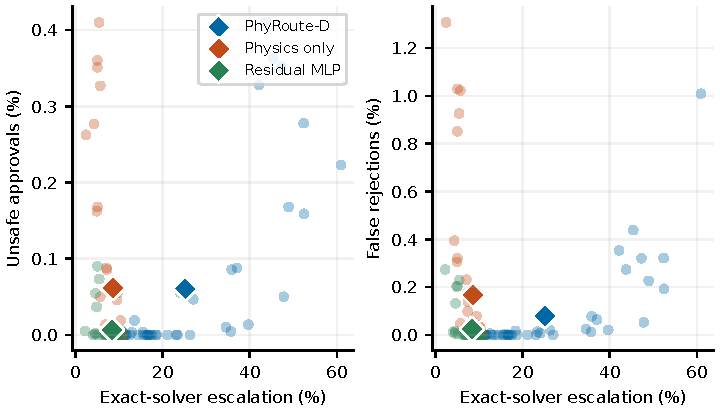
\includegraphics[width=\textwidth]{../figures/revised/nominal_tradeoff.pdf}
\caption{Three routes with current, correct physics at the frozen 10\% calibration setting. Faint points are means for individual held-out topologies; diamonds are the 44-topology macro means. Decision errors use resolved subsets and escalation uses all generated points. Stale neural routes are omitted to preserve the error scale.}
\label{fig:nominal}
\end{figure}

\subsection{Equal test budgets and nominal calibration}

At exactly 10\% retrospective test escalation, physics-only routing has an unsafe rate of 0.01326\% and a false-rejection rate of 0.04405\%. For the residual model, these rates are 0.00139\% and 0.00105\%. PhyRoute-D leaves 11.40195\% unsafe approvals, alongside 1.98871\% false rejections. Its frozen error rate depends on substantially increased escalation. Test-score quantiles diagnose ranking capacity and cannot replace calibration thresholds in a deployment claim.

Topology shift also differs from the tested operating-range shift. On the original topology, neural-margin, physics-only, residual and disagreement routes all have zero observed errors at the 10\% calibration setting. On the photovoltaic-growth test, neural-margin routing again has zero observed errors, while the residual route records 0.00556\% unsafe approvals. The residual model is therefore not uniformly superior across the two kinds of change.

The split-conformal route at $\alpha=0.001$ has no observed errors on either original-topology distribution, with 3.3011\% escalation in the nominal range. On held-out topologies its unsafe rate is 16.6929\% with the same 3.3011\% escalation. The unchanged rate follows the paired topology-blind inputs. This is a failure of transport to the changed conditional response, not a contradiction of the exchangeability-based conformal statement.

\subsection{The supplied verifier can also be wrong}

Table~\ref{tab:mismatch} and Fig.~\ref{fig:mismatch} hold physical truth fixed while changing the verifier. For the residual route, independent branch perturbations in $[0.9,1.1]$ increase the unsafe rate from 0.00647\% to 0.01039\%, with 0.04356\% false rejections. This single recorded perturbation is milder than a coherent bias and does not estimate performance averaged over possible network errors.

\begin{table}[tb]
\caption{Verifier mismatch with frozen nominal 10\% calibration thresholds. Entries give unsafe approvals / false rejections in percent, with the same macro averaging and denominators as Table~\ref{tab:nominal}. The physical reference is unchanged.}
\label{tab:mismatch}
\centering\small
\begin{tabular}{lrrr}
\toprule
Verifier & PhyRoute-D & Physics only & Residual MLP \\
\midrule
Correct & 0.061 / 0.079 & 0.061 / 0.168 & 0.006 / 0.025 \\
Branch noise $\pm10\%$ & 0.107 / 0.104 & 0.110 / 0.211 & 0.010 / 0.044 \\
$R,X\times0.80$ & 5.193 / 0.007 & 8.130 / 0.007 & 7.332 / $< 0.001$ \\
$R,X\times0.90$ & 2.308 / 0.021 & 3.143 / 0.024 & 2.243 / 0.002 \\
$R,X\times0.95$ & 0.918 / 0.040 & 1.102 / 0.061 & 0.334 / 0.007 \\
$R,X\times1.05$ & 0.013 / 0.161 & 0.014 / 0.366 & 0.002 / 0.933 \\
$R,X\times1.10$ & 0.005 / 0.517 & 0.005 / 2.702 & 0.001 / 5.031 \\
$R,X\times1.20$ & 0.002 / 1.814 & 0.002 / 11.489 & $< 0.001$ / 14.046 \\
Stale topology & 15.441 / 2.694 & 15.439 / 2.694 & 14.860 / 2.631 \\
\bottomrule
\end{tabular}
\end{table}


A coherent factor of 0.9 raises residual-route unsafe approvals to 2.24272\%; physics-only routing reaches 3.14304\% and PhyRoute-D reaches 2.30788\%. The residual model still improves the unsafe average over physics alone in this condition, but its nominal low-error level is lost. At factor 1.1, its unsafe rate falls to 0.001244\% while false rejections rise to 5.03135\%. Physics-only routing has 0.005498\% unsafe approvals and 2.70213\% false rejections. Depending on the direction of bias, conservative-looking voltage estimates can exchange missed violations for substantial rejection of feasible points.

\begin{figure}[tb]
\centering
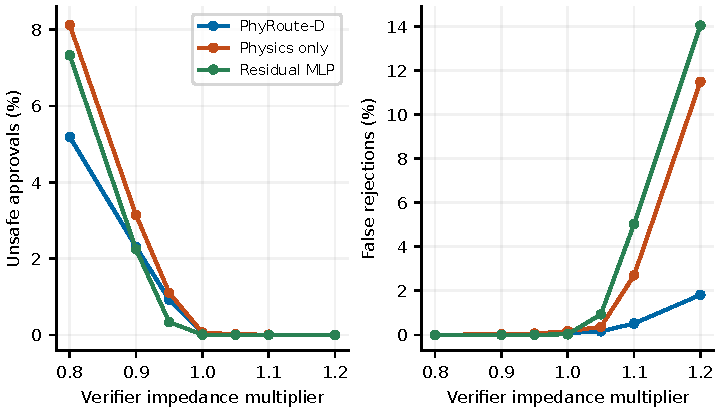
\includegraphics[width=\textwidth]{../figures/revised/impedance_sensitivity.pdf}
\caption{Sensitivity to coherent error in supplied line impedances, with reference physics and nominal calibration thresholds fixed. Ribbons span the three training-run means, not confidence intervals. Error percentages use resolved denominators. Lower unsafe approvals under overestimated impedance must be read alongside false rejections.}
\label{fig:mismatch}
\end{figure}

Using the stale original topology removes the useful current-network signal. Residual routing then has 14.85961\% unsafe approvals, versus 15.43925\% for physics-only routing and 15.44149\% for PhyRoute-D. The learned correction does not recover an omitted topology from operating features alone. The nominal result consequently supports a conditional benefit from supplied physical information, not immunity to verifier error.

\subsection{Complete-route computation}

Table~\ref{tab:latency} reports complete NumPy routes on an Apple M4 system with Python 3.11.14 and NumPy 2.4.6, with thread counts fixed to one. Timing uses training seed 4101 and test seed 9101, the original topology and the previously explored exchange \texttt{close35\_open31}. It covers varied batches of 1, 64 and 512, with two warm-ups, rotating method order and 200, 80 and 30 measured calls, respectively. These are declared resolved workloads with strict backward/forward-sweep fallback, not a measurement of Newton--Raphson retries on difficult reference cases.

\begin{table}[tb]
\caption{Measured complete-route mean latency in $\mu$s per scenario on an Apple M4 with one BLAS thread. Base is the original network; RC-A is the previously studied close35/open31 exchange. Batch size is shown in each column. Training seed 4101, test seed 9101; frozen 10\% calibration thresholds.}
\label{tab:latency}
\centering\small
\begin{tabular}{lrrrr}
\toprule
Route & Base, 1 & RC-A, 1 & Base, 512 & RC-A, 512 \\
\midrule
Always exact & 396.55 & 414.72 & 3.23 & 3.77 \\
Physics only & 64.04 & 57.81 & 1.34 & 1.46 \\
Neural margin & 91.88 & 93.00 & 1.98 & 2.13 \\
PhyRoute-D & 107.77 & 130.25 & 2.10 & 2.56 \\
Residual MLP & 74.45 & 66.32 & 1.57 & 1.72 \\
\bottomrule
\end{tabular}
\end{table}


For single-point calls on the original topology, mean time is 64.04~$\mu$s for physics-only routing, 74.45~$\mu$s for residual routing and 396.55~$\mu$s for always-exact evaluation. On the changed topology, the corresponding means are 57.81, 66.32 and 414.72~$\mu$s. The residual route's original-topology median is 29.85~$\mu$s and its p95 is 416.33~$\mu$s. Median single-point latency mostly reflects calls that skip fallback. Reporting it alone would understate workload cost and hide the fallback tail.

At batch size 512, original-topology mean times per scenario are 1.339, 1.570 and 3.226~$\mu$s for physics-only, residual and always-exact routes. The changed-topology means are 1.459, 1.721 and 3.769~$\mu$s. The residual model buys lower nominal decision errors with more computation than physics-only screening, despite its smaller escalation average in the held-out study. Lower escalation and lower latency are not interchangeable. Timing two topologies also cannot establish a latency bound across the inventory or an operational service-level guarantee.

\section{Discussion}
\label{sec:discussion}

\subsection{Information explains the topology-blind failure}

For a fixed trained predictor and routing score $g$, if the operating-feature distribution is unchanged between two topologies, the distribution of $g(X)$ is unchanged. For any measurable set $A$,
\begin{equation}
 P_{T_1}\{g(X)\in A\}
 =\int\mathbf{1}\{g(x)\in A\}\,dP_X(x)
 =P_{T_2}\{g(X)\in A\}.
\end{equation}
This is a direct observation about deterministic functions of the same inputs, not a new theorem. In the paired experiment, the scores agree pointwise across topologies. Labels can still differ because the voltage solution depends on the network. A stable confidence histogram therefore cannot be interpreted as evidence that the physical decision remains accurate.

LinDistFlow breaks that symmetry by receiving the supplied network. The residual model receives the same physical summary and learns corrections on development exchanges. Its held-out improvement over physics-only screening shows that a learned component can add useful discrimination once current information is supplied. A disagreement gate addresses the stale model differently: it routes its conflicts with physics for resolution. In this benchmark that can be expensive because the stale model itself generates many conflicts. The direct physics and residual routes need not preserve that stale verdict.

\subsection{What the comparison establishes}

The residual result is an empirical systems comparison with several differences between models. It uses 48,000 training points across development topologies, whereas the stale ensemble uses 30,000 points from the original topology. Its two hidden layers have 64 units each, and it is a single network rather than five 32-unit members. Current-physics inputs, training diversity, target parameterization, capacity and ensemble overhead all change together. The experiment does not isolate their individual causal effects. A claim that residual learning alone causes the gain would require matched ablations.

Under the stated training and calibration choices, the augmented route improves nominal error averages over the inexpensive verifier it uses. Runtime and mismatch results specify the price and conditions. Physics-only screening is simpler and faster in the measured routes. Where its remaining errors matter, learned correction offers a measurable alternative. No application-specific cost or acceptable-risk threshold was imposed after observing these outcomes.

Several limits remain. All exchanges derive from one balanced feeder, so held-out topology is not held-out network generalization. Synthetic load and photovoltaic ranges do not represent every operating regime. The random impedance experiment contains one realization per topology, and measurement error was not tested. Reference coverage remains incomplete on one topology. The revision followed an exploratory study, even though the expanded methods and allocation were frozen before the revised comparisons. These boundaries belong to the evidence, not to a claim of field readiness.

\section{Conclusion}

The strongest result is the measured value of correcting current LinDistFlow information before applying a calibrated fallback rule. On 44 held-out branch exchanges, that route reduces nominal unsafe approvals and false rejections relative to physics-only screening, with slightly less escalation but higher computation. Preserving a stale neural verdict through disagreement routing is less efficient at equal test capacity. Neither approach supplies a general safety certificate: coherent impedance error, stale topology and unresolved numerical cases limit the conclusion. A credible deployment comparison must account for the information each component receives, both decision errors, the realized solver workload and the conditions its reference cannot resolve.

\paragraph{Data and code.}
The companion reproducibility package contains the protocol and amendment, topology allocation, configuration and source hashes, non-executable model arrays, reference-coverage records, evaluation summaries and plotting and timing code. The original exploratory experiment is preserved separately.
% Public repository and archival identifiers await a verified release.

% AUTHOR ACTION: Human final review and approval of this disclosure are pending.
\paragraph{AI assistance.}
ChatGPT assisted with initial idea development. Claude developed the original experimental code and manuscript draft. Codex assisted with code and numerical audits, protocol revision, literature verification, revised experiment tooling, drafting and typesetting. Human authors retain responsibility for validating the evidence, interpreting the findings and approving the submitted text.
